\newpage
\pagestyle{empty}

\begin{minipage}[c]{.25\linewidth}
	
\includegraphics[width=4cm]{images/Logo-LEnsE.png}
\end{minipage} \hfill
\begin{minipage}[c]{.4\linewidth}

\begin{center}
\vspace{0.3cm}
{\Large \textsc{Opto-Electronique}}

\medskip

\textbf{\Large Ressources}

\end{center}
\end{minipage}\hfill

\vspace{0.5cm}

\noindent \rule{\linewidth}{1pt}
\section{Tracer la réponse en fréquence d'un système linéaire}
\label{ressource:RepFreq}


%%%%%%%%%%%%%%%%%%%%%%%%%%%%%%%%%%%%%%%%%%%%%%%%%%%%%%%%%%%%%%%%%%%%%%%%%%%%%%%%
%%%%%

La réponse en fréquence décrit la manière dont \textbf{un système réagit à différentes fréquences d'entrée}. Elle indique comment l'amplitude et la phase d'un signal sont modifiées lorsqu'il passe à travers un système ou un circuit, en fonction de la fréquence du signal.

Cette étude traduit le \textbf{comportement harmonique} d'un circuit, c'est à dire sa réponse à une excitation (en tension) sinusoïdale.

Cette fonction n'est définie que dans le cas de circuits linéaires. La tension de sortie est dans ce cas sinusoïdale et de même fréquence que le signal d'entrée.

\subsection{Objectif}

Obtenir l'allure de la \textbf{courbe du gain} et éventuellement de celle \textbf{du déphasage} apportés par le circuit en fonction de la fréquence du signal sinusoïdal placé en entrée.

Le \textbf{diagramme de Bode} est une manière spécifique de représenter la réponse en fréquence. Il s'agit d'une \textbf{représentation graphique} qui se compose de deux parties distinctes :

\begin{itemize}
	\item diagramme de Bode en gain (gain en $\operatorname{dB}$),
	\item diagramme de Bode en phase.
\end{itemize}

\bigskip

La courbe est souvent tracée avec une \textbf{échelle logarithmique} en fréquence. 

\subsection{Intérêt du passage en décibels (dB)}

Lorsqu'on cascade plusieurs systèmes entre eux, leurs fonctions de transfert se multiplient. Il n'est alors pas simple de pouvoir comparer \textbf{graphiquement} les systèmes à plusieurs étages facilement.

$$A = \prod_{k=1}^{n} A_k $$

En passant par une échelle logarithmique (en décibels par exemple), on transforme ce produit en une somme. Ainsi il sera plus simple de cumuler les effets d'une mise en cascade de systèmes linéaires et de voir le comportement global en additionnant les comportements de chacun des étages.

$$G_{dB} = \log(A) = \log(\prod_{k=1}^{n} A_k) = \sum_{k=1}^{n} \log(A_k) $$

\newpage
\subsection{Protocole d'étude}

\begin{itemize}
	\item Régler un \textbf{générateur de fonction} (ou GBF) pour avoir un \textbf{signal sinusoïdal} à sa sortie, avec une amplitude compatible avec les limites du circuit à tester.
	\item Relier le générateur de fonction à la fois à l'entrée du circuit et à une des entrées de l'oscilloscope.
	\item Relier la tension de sortie à une deuxième voie de l'oscilloscope.
	\item \textbf{S'assurer que le signal de sortie est bien sinusoïdal} avant d'aller plus loin. Dans le cas contraire, le système ne fonctionne pas de manière linéaire (amplitude trop élevée en entrée par exemple qui entraine une saturation en sortie...)
\end{itemize}


\section{Procédure classique}

Un premier balayage rapide en fréquence permet de \textbf{repérer les gammes de fréquences d'intérêt}.

Une analyse du \textbf{comportement du circuit pour les valeurs extrêmes de fréquences} (sur la phase et l'amplitude) apporte les informations sur le comportement asymptotique de la réponse en fréquence. Ce sont les \textbf{2 premiers points de mesure}.

\textbf{3 à 5 mesures supplémentaires} sont ensuite suffisantes :
\begin{itemize}
	\item l'une à la fréquence caractéristique du circuit, qui peut être : 
	\begin{itemize}
		\item la fréquence centrale d'un circuit passe-bande, 
		\item la bande passante à $-3\operatorname{dB}$ pour un circuit passe-bas ou passe-haut,
		\item la fréquence d'un déphasage particulier (en général la fréquence pour laquelle le déphasage apporté est égal à la moitié du déphasage maximal que le circuit peut apporter )
	\end{itemize}
	\item les autres de part et d'autres de cette fréquence caractéristique, à une octave au dessous (à la fréquence moitié) et une octave au dessus ( à la fréquence double)
\end{itemize}

\medskip

La figure~\ref{fig:rf_mesure} montre une capture d'écran d'oscilloscope d'un signal sinusoïdal $V_E$ appliqué à un système linéaire et sa sortie $V_S$. La méthode de mesure du gain du montage et du déphasage pour une fréquence particulière est représentée sur cette figure également.

\begin{figure}[h!]
    \centering
	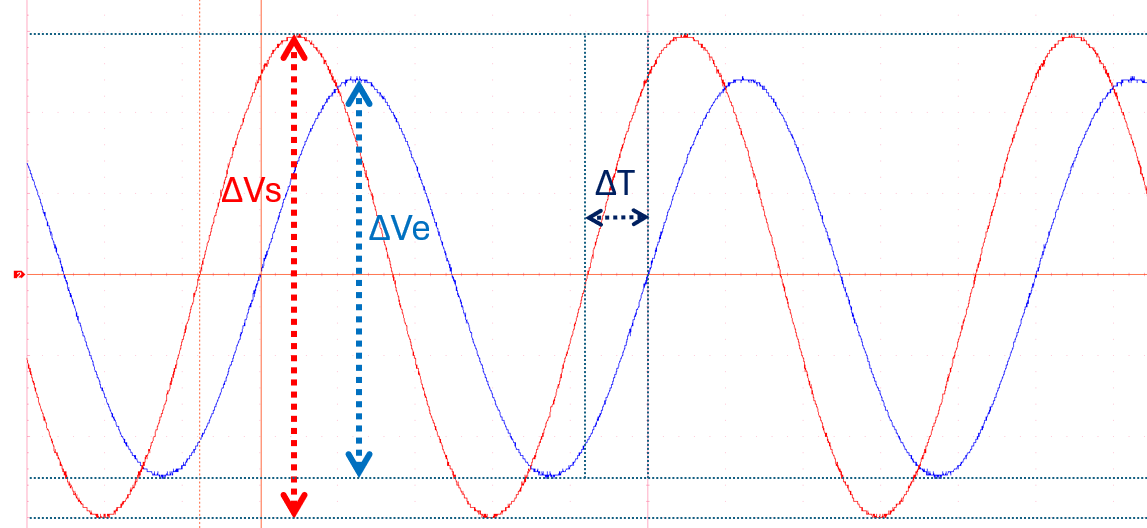
\includegraphics[width=0.8\textwidth]{images/rf_bode.png}
	
    \caption{Capture d'écran d'oscilloscope d'un signal sinusoïdal $V_E$ (en bleu) appliqué à un système linéaire et sa sortie $V_S$ (en rouge). Le calibre vertical est de 200mV/carreau pour $V_E$ et pour $V_S$. L'échelle horizontale est de 2ms/carreau.}
    \label{fig:rf_mesure}
\end{figure}

\newpage
\subsection{Mesure du gain du circuit}

Il existe \textbf{deux solutions pour déterminer la valeur du gain} :

\begin{itemize}
	\item Utiliser les mesures automatiques de l'oscilloscope, pour relever l'amplitude du signal d'entrée ($\Delta{}V_e$) et du signal de sortie ($\Delta{}V_s$), et utiliser un logiciel pour convertir le gain en $\operatorname{dB}$
	\item Utiliser le multimètre en dB-mètre (voir documentation annexe des instruments de mesure).
\end{itemize}

\medskip

On rappelle que le gain en décibel est égal à :

$$G_{dB} = 20 \cdot \log(A)$$

où $A = \frac{\Delta{}V_s}{\Delta{}V_e}$ est le gain du système.

\subsection{Mesure du déphasage}

Certains oscilloscopes proposent des mesures automatiques du déphasage. En leur absence, une mesure aux curseurs du décalage temporel $\Delta{}T$ entre les deux tensions (entrée et sortie) permet de remonter au déphasage $\Delta{}\phi$ par la formule :

$$\Delta{}\phi = +/- \frac{\Delta{}T}{T} \cdot 2\pi$$

où T est la période du signal.

Il est important de déterminer lequel des deux signaux est en avance sur l'autre, afin de donner un signe au déphasage apporté par le circuit. Si la tension de sortie est en retard sur la tension d'entrée, le déphasage est négatif.

\newpage
\section{Allure rapide}

Il existe également une \textbf{méthode automatique} pour obtenir l'allure de la réponse en fréquence du système, selon le modèle de GBF que vous possédez.

En effet, certains d'entre eux sont capables de réaliser automatiquement un balayage en fréquence.

Pour les GBF \textbf{\texttt{Agilent}} (des salles de TP d'électronique, par exemple), il faut utiliser au préalable sélectionner un \textbf{signal sinusoïdal}, de n'importe quelle fréquence mais d'amplitude et de valeur moyenne (offset) compatible avec le système à étudier (si ALI/AOP, vérifiez que le signal de sortie ne sature pas, par exemple).

Puis sélectionner ensuite le menu \textbf{Sweep} du GBF. Se référer ensuite à la documentation du GBF fournie sur vos paillasses pour les réglages (voir aussi figure~\ref{fig:gbf_sweep}).

\begin{figure}[h!]
    \centering
	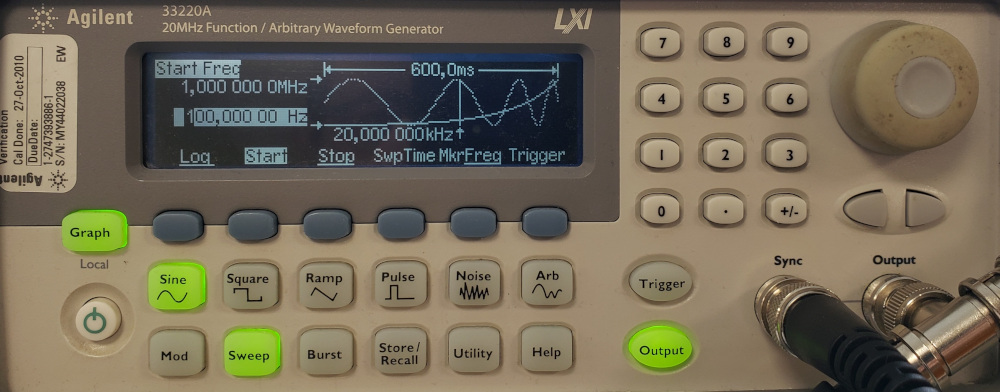
\includegraphics[width=0.6\textwidth]{images/gbf_sweep.jpg}
	
    \caption{Photographie d'un générateur de fonction Agilent 33220A en mode \textit{sweep} (balayage).}
    \label{fig:gbf_sweep}
\end{figure}


Il est ensuite possible de synchroniser l'oscilloscope avec le GBF en utilisant la sortie \textbf{Sync}, qui fournit un signal rectangulaire de même période que le balayage, connectée à l'une des entrées de l'oscilloscope (EXT si on ne souhaite que synchroniser) et en réglant les paramètres du déclenchement de l'oscilloscope.

\begin{figure}[h!]
    \centering
	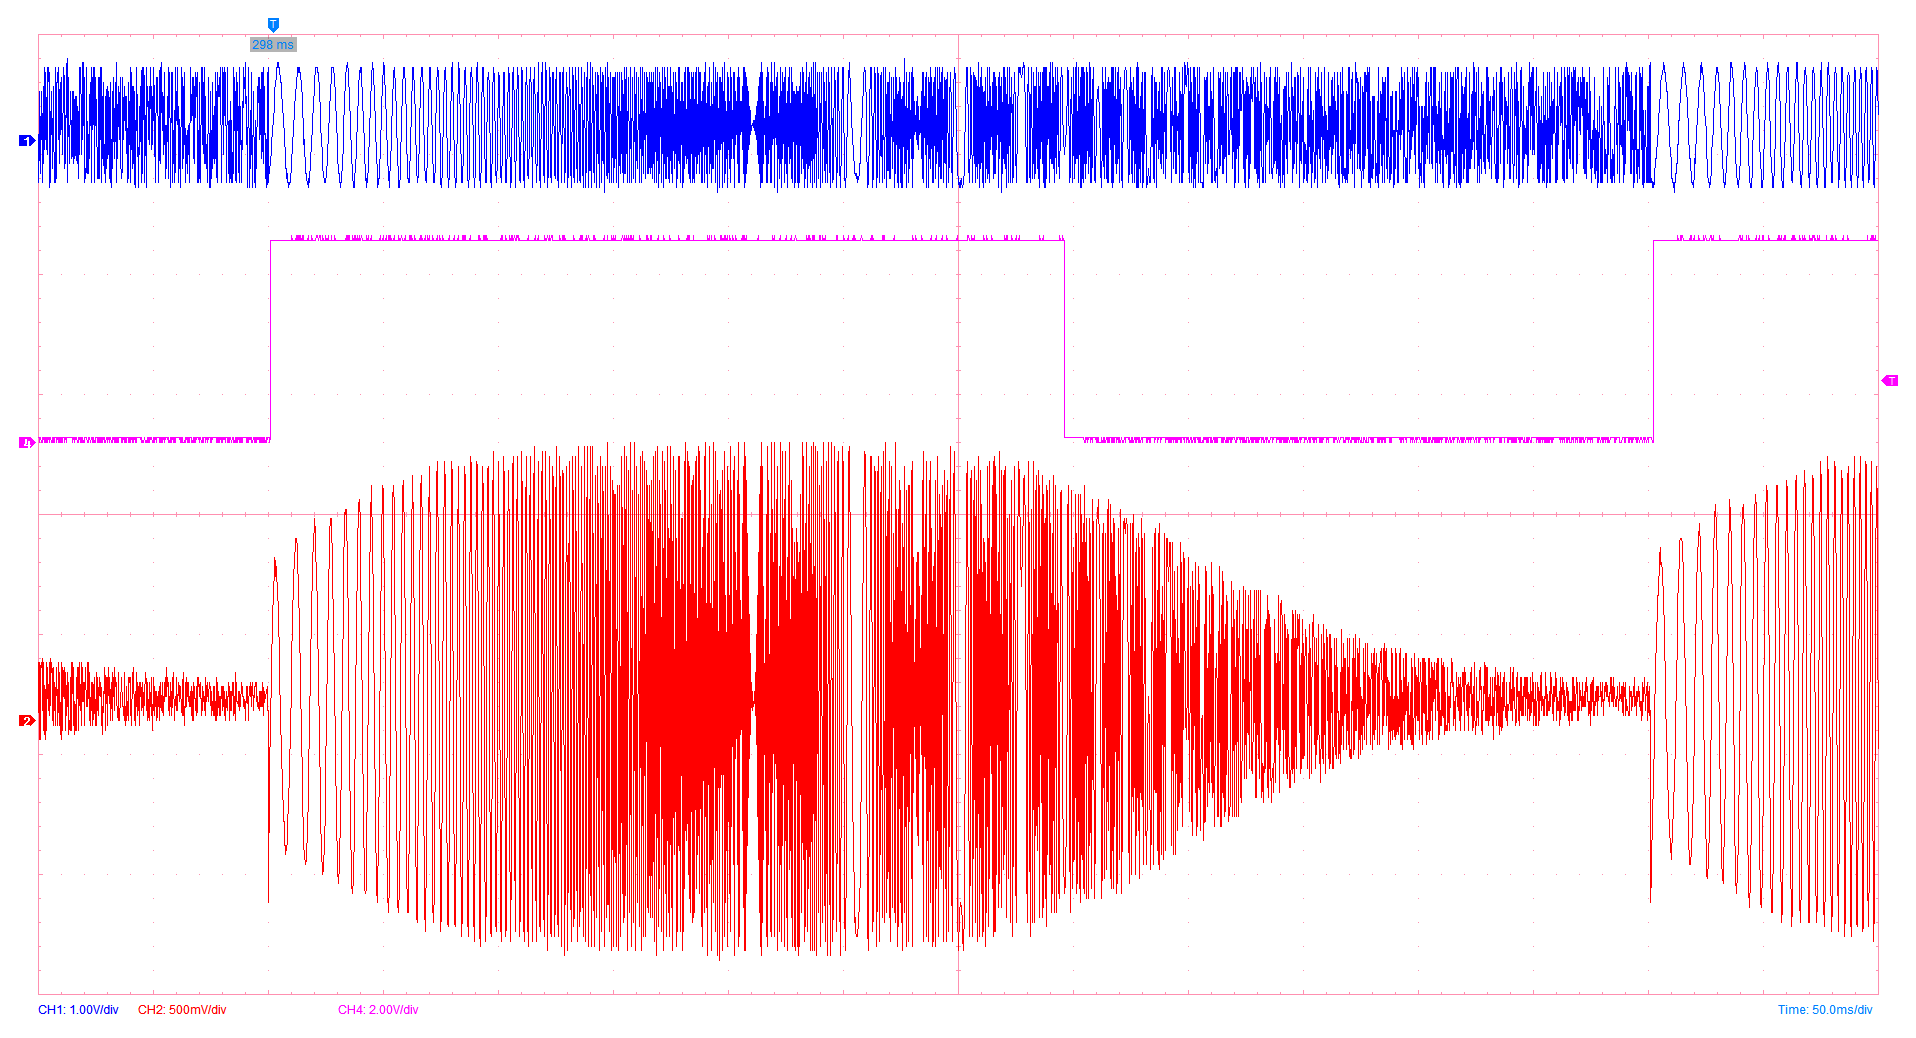
\includegraphics[width=0.7\textwidth]{images/gbf_sweep_sync.png}
	
	%Cas d'un passe-bande - en haut signal d'entrée (amplitude constante), au centre signal de synchronisation (avec marqueur en fréquence - retour à l'état bas) et en bas signal de sortie.

	
    \caption{Capture d'écran d'oscilloscope d'un balayage en fréquence $V_E$ (en bleu) appliqué à un système linéaire et sa sortie $V_S$ (en rouge) - cas d'un passe-bande. En haut signal d'entrée $V_E$ (amplitude constante), au centre signal de synchronisation (avec marqueur en fréquence - retour à l'état bas) et en bas signal de sortie $V_S$. Le calibre vertical est de 1V/carreau pour $V_E$ et de 200mV/carreau pour $V_S$. L'échelle horizontale est de 50ms/carreau.}
    \label{fig:rf_sweep}
\end{figure}

\newpage
\section{Quelques rappels}
%%%%%%%%%%%%%%%%%%%%%%%%%%%%%%%%%%
\subsection{Déphasage}

En régime harmonique (à même fréquence), deux ondes sinusoïdales peuvent avoir des phases initiales différentes.

Soient $u_1(t) = A_1 \cdot sin(2\pi f t + \varphi_1)$ et $u_2(t) = A_2 \cdot sin(2\pi f t + \varphi_2)$, le déphasage de l'une par rapport à l'autre à l'instant $t$ vaut : $\Delta\varphi = (2\pi f t + \varphi_2) - (2\pi f t + \varphi_1) = \varphi_2 - \varphi_1$

\medskip

Si $\Delta\varphi$ est positif, l'onde 2 est en avance de phase par rapport à l'onde 1. Sinon, l'onde 2 est en retard de phase par rapport à l'onde 1.

%%%%%%%%%%%%%%%%%%%%%%%%%%%%%%%%%%
\subsection{Phase et ordre d'un filtre}

Lorsqu'on étudie des systèmes linéaires de type filtre, il est intéressant de relever le déphasage entre le signal de sortie et le signal d'entrée pour différents points remarquables :

\begin{itemize}
	\item à la fréquence caractéristique du système, le déphasage est égal à $k\cdot \pi/4$ où $k$ est un entier correspondant à l'ordre du filtre
	\item loin de cette fréquence caractéristique (au moins une décade avant et après), pour vérifier le caractère inverseur d'un système par exemple.
\end{itemize}
